\section{Leaks}
We can use the same techniques we have learned so far for leaked information.
However, the focus here is on information that only employees are likely to
have. The word "leak" refers to a source of leakage in companies,
organizations, and governments. In this case, information is disclosed that is
not intended for public consumption. This information can still be damaging,
regardless of the company's infrastructure.
\begin{figure}
  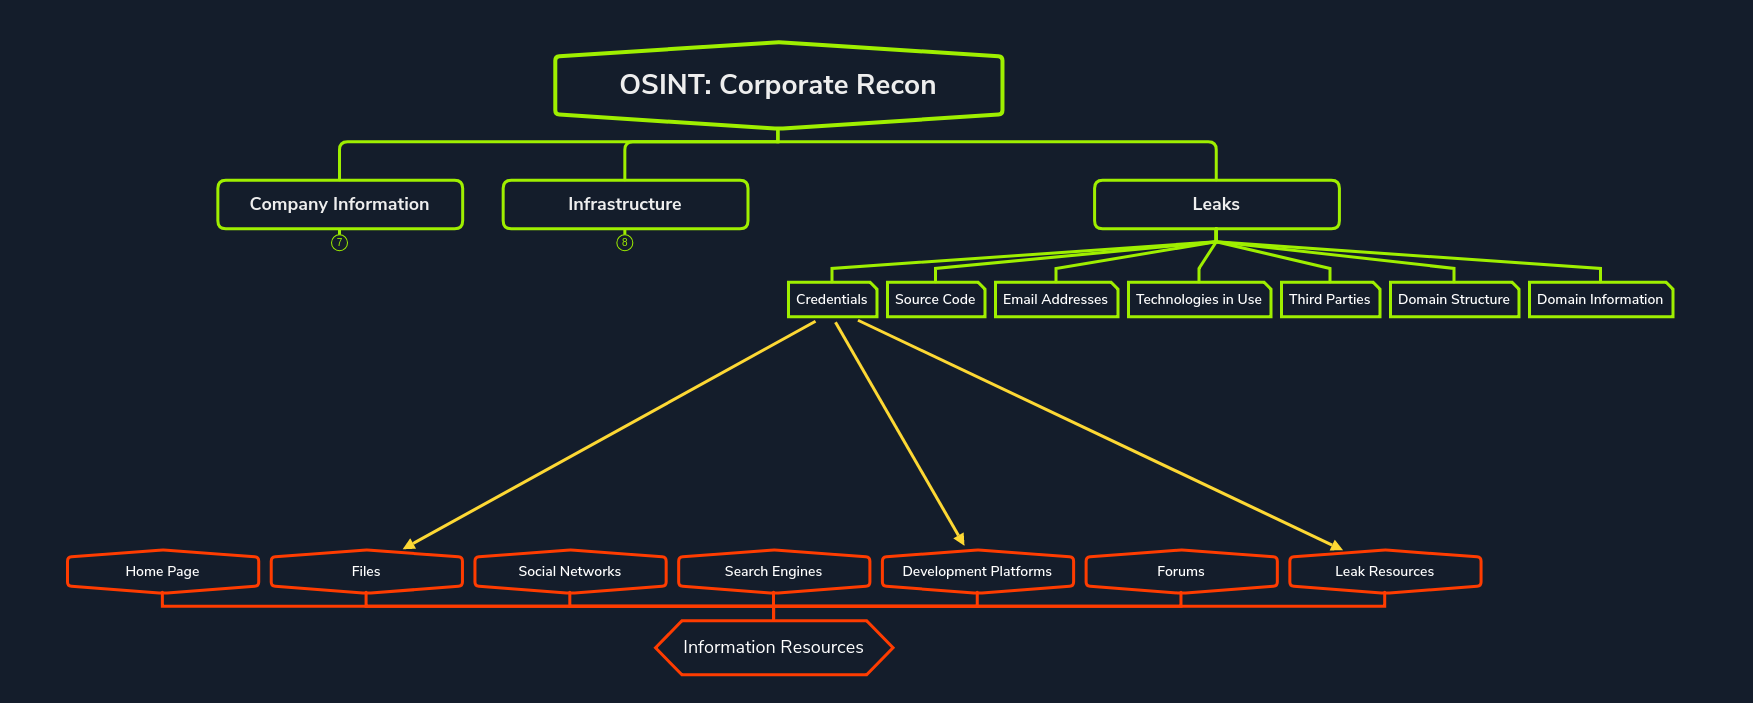
\includegraphics[width=\linewidth]{recon/osint/images/leaks.png}
  \caption{OSINT Leaks}
  \label{fig:osint-leaks}
\end{figure}
Leaks are not only made by attackers but also by the company's own employees.
If it is an employee, the cause of such information disclosure can be either
{\bf accidental} (through carelessness), {\bf intentional}, or {\bf forced}. In
the third case, it is a lose-lose situation into which one has been forced and
in which there is usually time pressure.

{\bf Accidental leaks} represent a disclosure of information and data that, in
most cases, is intended for internal purposes only. This is done only by the
employees of the company for many reasons. Generally, accidental leaks are
referred to as {\bf information disclosure}.

To illustrate this as thoroughly as possible, we can imagine source code that
contains commented-out credentials that the developers have inserted for
convenience. Suppose, however, and we find these credentials in the source
code, which is an essential part of its function. In that case, it is
information disclosure and no longer refers to the contents of the code but
access rights (and thus to the administration and configuration of the
system).


{\bf Intentional leak} takes place purposefully and always has the goal of
making secret, confidential or private data public. With a leak, an insider
wants to expose dishonorable, immoral, unethical behavior and make it
accessible to the public. In some cases, attackers want to cause damage with a
leak.

If we go back to our previous example and assume the developer added those
credentials there on purpose and the intent for harm, then this is a leak.

In a leak, rules and laws are deliberately broken. Because at its core, a leak
is data theft and violates confidentiality agreements. A leak becomes possible
when an internal employee violates the trust and security rules given to them.
For attackers, a leak requires them to find software vulnerabilities to steal
data. A leak can occur by an insider who had legitimate access to the data, but
it does not have to. Websites or social media profiles can also be hacked by
outsiders, allowing data to be stolen. The insider, also known as a
whistleblower, remains anonymous to avoid prosecution.


A {\bf forced leak} means that the person or organization concerned often has
no way to avoid the prospective personal or cooperative damage. This type of
disclosure usually involves blackmailing the person or organization concerned.
This is often the modus operandi of various malware activities that force the
person or organization to pay with money or specific activities, or the
encrypted/stolen data is kept and published. These are cases where {\bf Digital
Forensics and Incident Response (DFIR)} is used to identify the attackers and
undo the damage caused by the malware.

The source of a leak can be any conceivable information resource. We can see
how efficient our methodology is since we no longer base our information
gathering approach on information resources but on the categories of
information we want. Here we examine the information resources already found
for the data for each category. There are information resources designed to
find this type of content, and these are divided into three fields, {\bf
archives}, {\bf internal leaks}, and {\bf breaches}.

\subsection{Archives}

An archive represents anything that contains an enormous amount of written
information in some structured form and is not a library. It is therefore used
to store information that can be accessed (un)restricted. An archive,
therefore, stores information about the required information resource at
specific intervals with special conditions. From 1999, it has been extended by
other archives, so it is now a digital library that includes significant
collections of texts and books, audio files, videos, images, and software. The
Internet Archive is dedicated to the long-term archiving of digital data in a
freely accessible form.

Besides the already mentioned forums and social media platforms, archives
should not be left out. These archives, such as
\href{https://archive.org/}{WayBack Machine} or
\href{http://archive.fo/}{Archive.fo}, create so-called snapshots or captures
of websites and store images, videos, audio recordings, software, and files
that have been published on the websites.

These captures of web pages are taken by a crawler. In 2018 the WayBack Machine
archived over 380 billions of web pages. Viewing older versions of these sites
also allows us to see and analyze the source code. This can include, for
example, the robots.txt of a web server, which may indicate hidden folders on
the webserver that still exist.

We can also display URLs that the WayBack Machine has crawled. Here it is often
shocking how many URLs are publicly accessible even if we think that the
published information from the past no longer exists. We may also find content
that has been removed by our target company for security reasons, for example,
that describes their technology in too much detail or even reveals other
information such as their internal processes.

Another interesting feature of WayBack Machine is that it also shows us in the
Summary how many new links it has captured compared to the previous year. Here
we get an overview of potentially existing folders and files that are now
hidden from the public but still exist for further development or as a backup
on the system. These can be detected using the filter located at the top right
above the table. There we can enter the file extensions that are being searched
for. Applications and administrators use many different file extensions. A list
of them can be found at
\href{https://fileinfo.com/filetypes/backup}{FileInfo.com}.


Another critical information resource is
\href{https://pastebin.com/}{Pastebin.com}. There, different people share
information in text form with each other. Pastebin is a web application that
acts as a kind of online clipboard and can store any text, even large text
blocks, on the web and make it accessible to third parties via a link. The
interesting feature of the tool is that it supports syntax highlighting for
many programming languages. This makes the code much more convenient to read
and easier to understand. Since this feature, which is crucial for programmers,
is missing from most blogs, social networks, forums, or chat programs, it has
been reported that there are now over 15 million "pastes" on the website.
Pastebin now offers some options not to save the shared information
permanently. These include setting a password, which in most cases are
relatively weak, and the Burn after reading function, which deletes the content
after viewing. As we have done in previous search engine searches, we can also
narrow down the results using the \verb+site:+ dork to the Pastebin page, giving us
some impressive results.

\begin{verbatim}
site:pastebin.com XXX password router
\end{verbatim}

he art of finding this type of information is to combine the different
information that we already know. To efficiently discover these leaks, the
research we have done in the previous sections is necessary. Otherwise, we
would be blindly searching for leaks on the off chance that our search might
take an incalculably long time and even yield no results.

\subsubsection{Internal Leaks}
Most employees who create and edit documents and are not familiar with IT
security may not know which data will be published even under certain
conditions. They are cautious about what they write in the document. Still,
they don't know that it is not always necessary to write sensitive data in the
documents, whether it contains information about the company's working
environment.

Almost all websites have their own images, files, documents, and notes which
they make available to the visitors. In most cases, these were created or at
least edited on computers. Whenever files are modified, so-called metadata is
written to the resulting files. These often contain the name of the application
that was used for it and sometimes its version. Even some operating systems
write their own metadata into these files.

For a regular user, this data is irrelevant. Still, it gives us an excellent
insight into the employees' working environment and the software they are using
along with the versions.

One of the most effective and most comfortable to use tools is Exiftool. On the
website of our target company, we could find some reports which are available
for download. We can take advantage of them, download them, and examine these
reports to determine if specific metadata has been added to the files.
\begin{verbatim}
exiftool document.pdf
\end{verbatim}

We already know which software and version were used to create this document
from the downloaded document without looking at its contents. We also see
precisely when this document was created and last edited. We can also see the
PDF version, encryption type, language, operating system used to create this
document, and other valuable information.

Since we know that specific software tends to insert its metadata into files,
we must be careful how we download the files from our target company. Often,
when we download images using Firefox, we can see that the metadata, such as
the date and time of creation, may differ from actual values. It is therefore
recommended to download these files via wget to avoid accidentally manipulating
the metadata.

Internal leaks include almost any file from which we can extract metadata.
However, other sources may reveal internal information. The more we analyze the
company, the better we learn to understand its structure. This gives us a
variety of results, which can lead to internal calendars.

Calendars contain not only the date and time of certain events, but also names,
email addresses, locations, topic content, links, and other information. This
makes them very valuable, as it is assumed that no third party can access this
information.

Not only metadata and poorly hidden internal applications can provide us with
valuable information but also whole software or code published on
\href{https://github.com/}{Github} or \href{https://gitlab.com/}{Gitlab}. This
content can also contain security-related information that developers have
forgotten to remove.

\subsubsection{Breaches}

When we talk about breaches, we mean any documentation of existing losses of
information. Apart from various news like the attack on
\href{https://www.cnet.com/news/solarwinds-hack-officially-blamed-on-russia-what-you-need-to-know/}{SolarWinds},
many databases contain more detailed information about it. These include
descriptions of vulnerabilities and even {\bf Proofs-of-Concept (POCS)}. One of
the largest databases for stolen passwords with the respective email addresses
is "\verb+Collection #1-5+". 

We have already seen the resource, \href{Have I Been Pwned?} (HIBP). This
resource works exactly with this database to determine if the given email
address is stored there. If we work with offline cracking, HIBP offers us the
possibility to download huge password lists since these lists are excellent for
cracking password-protected files or hashes that we find during our penetration
test. The probability of current passwords being used repeatedly is very high.
Of course, we should try smaller lists and self-generated lists before using
~11 GB lists.

From the previous metadata, we could determiethe version of Acrobat. There
exist also databases where already known vulnerabilities are published. Such
databases are, but not limited to:
\begin{verbatim}
https://www.cvedetails.com/
https://www.exploit-db.com/
https://vuldb.com/
https://cve.mitre.org/
https://www.securityfocus.com/
\end{verbatim}

Breaches also include the so-called 0-days and N-days exploits. 0-day exploits
are publicly published vulnerabilities that the software providers have not yet
fixed. N-day exploits represent ways to exploit the targets that have not yet
patched the publicly known vulnerabilities. This means that although a patch or
update for the specific vulnerability exists, it has not yet been applied. When
we talk about breaches, we mean any documentation of existing losses of
information. Apart from various news like the attack on SolarWinds, there are
also many databases that contain more detailed information about it. These
include descriptions of vulnerabilities and even Proofs-of-Concept (POCs)., the
company has not yet updated the software.

0-days and N-days exploits can often be found on IT security forums as well as
on the deep-web or dark-web. These are often auctioned off, and the companies
themselves are also willing to pay a lot of money to find out what the
vulnerability looks like. This gives them a direct insight into the
vulnerability and an idea of how to patch it.

Many applications and operating systems are often not updated, as this could
harm the functionality of the business workflow. As a result, many
administrators risk leaving outdated software and potential vulnerabilities in
place rather than dealing with updates and patches that could shut down the
entire business workflow.

After all, we don't think about how vulnerable an application, which is less
than one year old, can be. In other Modules we will learn how quickly
vulnerabilities can be found in new applications.
